\let\negmedspace\undefined
\let\negthickspace\undefined
\documentclass[journal]{IEEEtran}
\usepackage[a4paper, margin=10mm, onecolumn]{geometry}
\usepackage{lmodern} % Ensure lmodern is loaded for pdflatex
\usepackage{tfrupee} % Include tfrupee package

\setlength{\headheight}{1cm} % Set the height of the header box
\setlength{\headsep}{0mm}  % Set the distance between the header box and the top of the text

\usepackage{gvv-book}
\usepackage{gvv}
\usepackage{cite}
\usepackage{amsmath,amssymb,amsfonts,amsthm}
\usepackage{algorithmic}
\usepackage{graphicx}
\usepackage{float}
\usepackage{textcomp}
\usepackage{xcolor}
\usepackage{txfonts}
\usepackage{listings}
\usepackage{enumitem}
\usepackage{mathtools}
\usepackage{gensymb}
\usepackage{comment}
\usepackage[breaklinks=true]{hyperref}
\usepackage{tkz-euclide} 
\usepackage{listings}
% \usepackage{gvv}                                        
\def\inputGnumericTable{}                                 
\usepackage[latin1]{inputenc}                                
\usepackage{color}                                            
\usepackage{array}                                            
\usepackage{longtable}                                       
\usepackage{calc}                                             
\usepackage{multirow}                                         
\usepackage{hhline}                                           
\usepackage{ifthen}                                           
\usepackage{lscape}
\usepackage{tikz}
\usetikzlibrary{patterns}

\begin{document}

\bibliographystyle{IEEEtran}
\vspace{3cm}

\title{4.13.68}
\author{EE25BTECH11064 - Yojit Manral}

\maketitle
% \maketitle
% \newpage
% \bigskip
{\let\newpage\relax\maketitle}
\renewcommand{\thefigure}{\theenumi}
\renewcommand{\thetable}{\theenumi}
\setlength{\intextsep}{10pt} % Space between text and float

\textbf{Question:}\\
Prove or disprove: The straight line $5x + 4y = 0$ passes through the point of intersection of the straight lines $x + 2y - 10 = 0$ and $2x + y + 5 = 0$.

\textbf{Solution:}\\
$\rightarrow$ Let
\begin{align*}
    \vec{n_1}^T\vec{x} = c_1 && \vec{n_2}^T\vec{x} = c_2 && \vec{n_3}^T\vec{x} = c_3
\end{align*}
\hspace{0.3cm} where
\begin{align}
    \vec{n_1} = \myvec{5\\4} && c_1 &= 0 \\
    \vec{n_2} = \myvec{1\\2} && c_2 &= 10 \\
    \vec{n_3} = \myvec{2\\1} && c_3 &= -5
\end{align}
$\rightarrow$ The three lines are concurrent if there exists some $\vec{x}$ such that
\begin{align}
    \myvec{\vec{n_1}^T\\\vec{n_2}^T\\\vec{n_3}^T} \vec{x} &= \myvec{c_1\\c_2\\c_3} \\
    \vec{A}\hspace{0.35cm}\vec{x} &= \hspace{0.2cm}\vec{B}
\end{align}
$\rightarrow$ A unique $\vec{x}$ exists iff the matrix $\vec{A}$ is a full-rank matrix (i.e., rank 2 for a system of 2 variables).
\begin{align}
    \vec{A} = \myvec{5&4\\1&2\\2&1}
    &\xrightarrow[R_2 \leftrightarrow R_2 - R_1]{R_1 \leftrightarrow (1/5)R_1} \myvec{1&4/5\\0&6/5\\2&1}\\
    &\xrightarrow[R_2 \leftrightarrow (5/6)R_2]{R_3 \leftrightarrow R_3 - 2R_1} \myvec{1&4/5\\0&1\\0&-3/5}\\
    &\xrightarrow[R_1 \leftrightarrow R_1 - (4/5)R_2]{R_3 \leftrightarrow R_3 + (3/5)R_2} \myvec{1&0\\0&1\\0&0}
\end{align}
\begin{align*}
    \text{Only 2 nonzero rows in the matrix in (8)}
    &\longrightarrow \text{Rank of the matrix $\vec{A}$ is 2} \\
    &\longrightarrow \text{$\vec{A}$ is a full rank matrix} \\
    &\longrightarrow \text{A unique $\vec{x}$ exists which satisfies all equations} \\
    &\longrightarrow \text{The three lines are concurrent}
\end{align*}
\begin{figure}[h!]
   \centering
   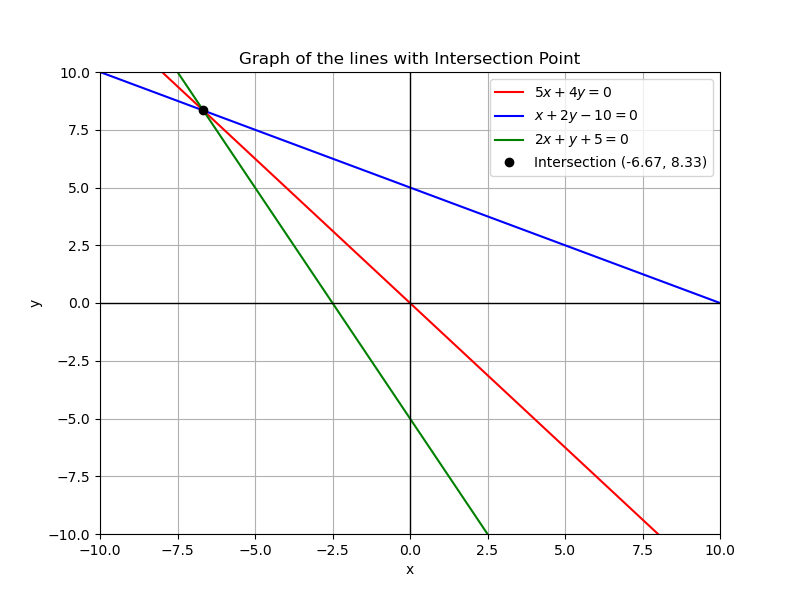
\includegraphics[width=\linewidth]{figs/01.png}
   \caption{Plot of the three lines}
   \label{Plot_1}
\end{figure}
\end{document}
